%\documentclass[a4paper, 12pt]{report}
\documentclass[]{article}
\usepackage[paperwidth=400pt, paperheight=300pt, margin=40pt]{geometry}

\usepackage[utf8]{inputenc} 

\usepackage[pdftex]{graphicx}
\graphicspath{{obr/}}
\DeclareGraphicsExtensions{.pdf, .jpg}

%\usepackage[slovak]{babel}

\usepackage{amsmath}

\usepackage[breaklinks]{hyperref}

\usepackage{lettrine}

\usepackage{microtype}

\usepackage{placeins}

\usepackage{fourier}
\usepackage{Baskervaldx}	% funguje aj smallcaps: \textsc 

\pagestyle{headings}

%% velkost fontu pod obrazkom mensia, vratane ``Obr. X:''
%\renewcommand{\figurename}{sjls} % toto nefunguje pri pouzivani babel
%\addto\captionsslovak{\renewcommand{\figurename}{\small Obr.}}
%\addto\captions{\renewcommand{\figurename}{\small Obr.}}
\renewcommand{\figurename}{\small{Figure}} % toto nefunguje pri pouzivani babel
\renewcommand{\thefigure}{\small \arabic{figure}}


\newcommand{\dif}{\, \mathrm{d}}	% diferencia (na derivacie)
\newcommand{\difp}{\partial}		% parc. diferencia 
\newcommand{\dxdt}[2]{\frac{\mathrm{d} #1}{\mathrm{d} #2}}
\newcommand{\dxdtp}[2]{\frac{\partial #1}{\partial #2}}
\newcommand{\un}[1]{\, \mathrm{#1}}	% jednotky velicin, v math mode
\newcommand{\E}[1]{\cdot 10^{#1}}
\newcommand{\degree}{^\circ}
\newcommand{\diameter}{\emptyset}
\newcommand{\cpx}{\widehat}		% komplexne fazory
\newcommand{\Ohm}{\Omega}


\newcounter{myasscount}
\renewcommand{\themyasscount}{\alph{myasscount}}
%\setcounter{myasscount}{1}
\newenvironment{myass}
{

	\refstepcounter{myasscount}
	\par
	\vspace{6pt}
	%\indent	% netreba, ked predchadza \par
	\begin{tabular}{p{.22\textwidth}  p{.68\textwidth} }
	\textbf{Predpoklad (\themyasscount)}	&
}
{
	\end{tabular}
	\par 
	\vspace{6pt}
}

\newcommand{\myfig}[3]
{
    \begin{figure}[!ht]
	\centering
	\includegraphics{#1}
	\caption{#2}
	\label{fig:#3}
    \end{figure}
}

\newcommand{\myfigd}[2]
{
    \begin{figure}[!htb]
	\centering
	\hspace{1.5mm}\includegraphics[height=.4\textheight]{./obr/plots_stat/#1}
	\hspace{11.5mm}\includegraphics[height=.4\textheight]{./obr/plots_stat/#1}\\\vspace{5mm}
	\includegraphics[height=.4\textheight]{./obr/plots_stat/bar}
	\hspace{10mm}\includegraphics[height=.4\textheight]{./obr/plots_stat/bar}
	\caption{$600\un{V}$, $40\un{A}$, $25\un{\degree C}$}
	%\label{fig:#3}
    \end{figure}
}


\begin{document}

\author{Ján Mikláš}
\date{Rožnov p. Radhoštěm, May 2016}
\title{\vspace{1cm} \textsc{Characterization of ``Handmade-packaged'' IGBT Chips}\\\rule{.5\textwidth}{1pt}\\Internship Report}


\maketitle

\newpage
\tableofcontents

\newpage
\section{Motivation} \label{sec:motivation}

To gain time \& resources economization, the ability to characterize the testing dies directly in place of developement in Rožnov would be beneficial.

Several ``packaging'' and measurements options are dealt with in this document as well as observed impact on the device characteristics.


\newpage
\section{Packaging} \label{sec:packaging}

%\begin{minipage}{.7\textwidth}
\begin{itemize}
    \item Wire bonding 
	\begin{itemize}
	    \item max. $\diameter 1\un{mil} \,\,(\approx 25\un{\mu m})$\footnote{CRESSTO s.r.o., Rožnov p. R., \url{www.cressto.cz}}\footnote{SEANT Technology s.r.o., Brno, \url{www.seant.cz}} contrary to $15\un{mil}$ used for IGBTs
	    \item max. continuous current $\approx 1\un{A/1wire}$; 8 wires tested as sufficient for double pulse current over $80\un{A}$
	\end{itemize}
    \item encapsulation: epoxy resin - availability and simple treatment
	\begin{itemize}
	    \item dilatation harmless even for bond wires of $\diameter 1\un{mil}$
	\end{itemize}
\end{itemize}
%\end{minipage}

%\begin{minipage}{.3\textwidth}
\begin{figure}[!ht]
    \centering
    \vspace{.3\textheight}
    \includegraphics[height=.4\textheight]{pkg_be}
    \includegraphics[height=.4\textheight]{bond1}
    \includegraphics[height=.4\textheight]{bond2}
    \caption{``TO247'' package before epoxy encapsulation.}
    \label{fig:pkg_be}
\end{figure}
%\end{minipage}


\newpage
\section{Measurements} \label{sec:measurements}

\subsection{Switching - Double-pulse Test}
\includegraphics{DP_schema}
\includegraphics[height=.9\textheight, width=.5\textwidth]{DP_waveforms}

\subsection{IV-curves}
\begin{itemize}
    \item temperature dependence
    \item low voltage ($20\un{V}$) induction load pulse test
    \item requires precise $V_{CE,sat}$ and $I_C$ sensing
\end{itemize}

\subsection{BV test}
\begin{itemize}
    \item Tektronix 370A, Programmable Curve Tracer
\end{itemize}

\includegraphics[width=.34\textwidth]{curve_tracer}


\newpage
\section{Strucured Processing of Measured Data}

\begin{itemize}
    \item exporting or manually editing ASCII (.csv) datafiles from oscilloscope (BV tester, etc.)
    \item data reading, processing and plotting/exporting using \textit{Octave} (\textsc{Matlab})
	\begin{itemize}
	    \item {useful functions library attached}
	\end{itemize}
\end{itemize}

\subsection{Data processing flowchart}
(please see the attached functions library for detail and expamples)

\includegraphics[height=\textheight]{data_processing_diagram}
\newpage
\includegraphics[height=\textheight]{data_processing_diagram_wafers}


\newpage
\section{Measurements Results }
\footnote{needs to be completed}

\subsection{Switching}
\begin{itemize}
    \item time intervals defined according to Figure \ref{fig:def_off} and Figure \ref{fig:def_on}
    \item sandwich DC link - $V_{peak,off}$ reduced to $\approx 50\un{V}$ (previously $\approx 120V$)
    \item fast SiC freewheeling diode - $i_{peak,on}$ reduced significantly
	
\end{itemize}

\begin{figure}[ht!]
    \centering
    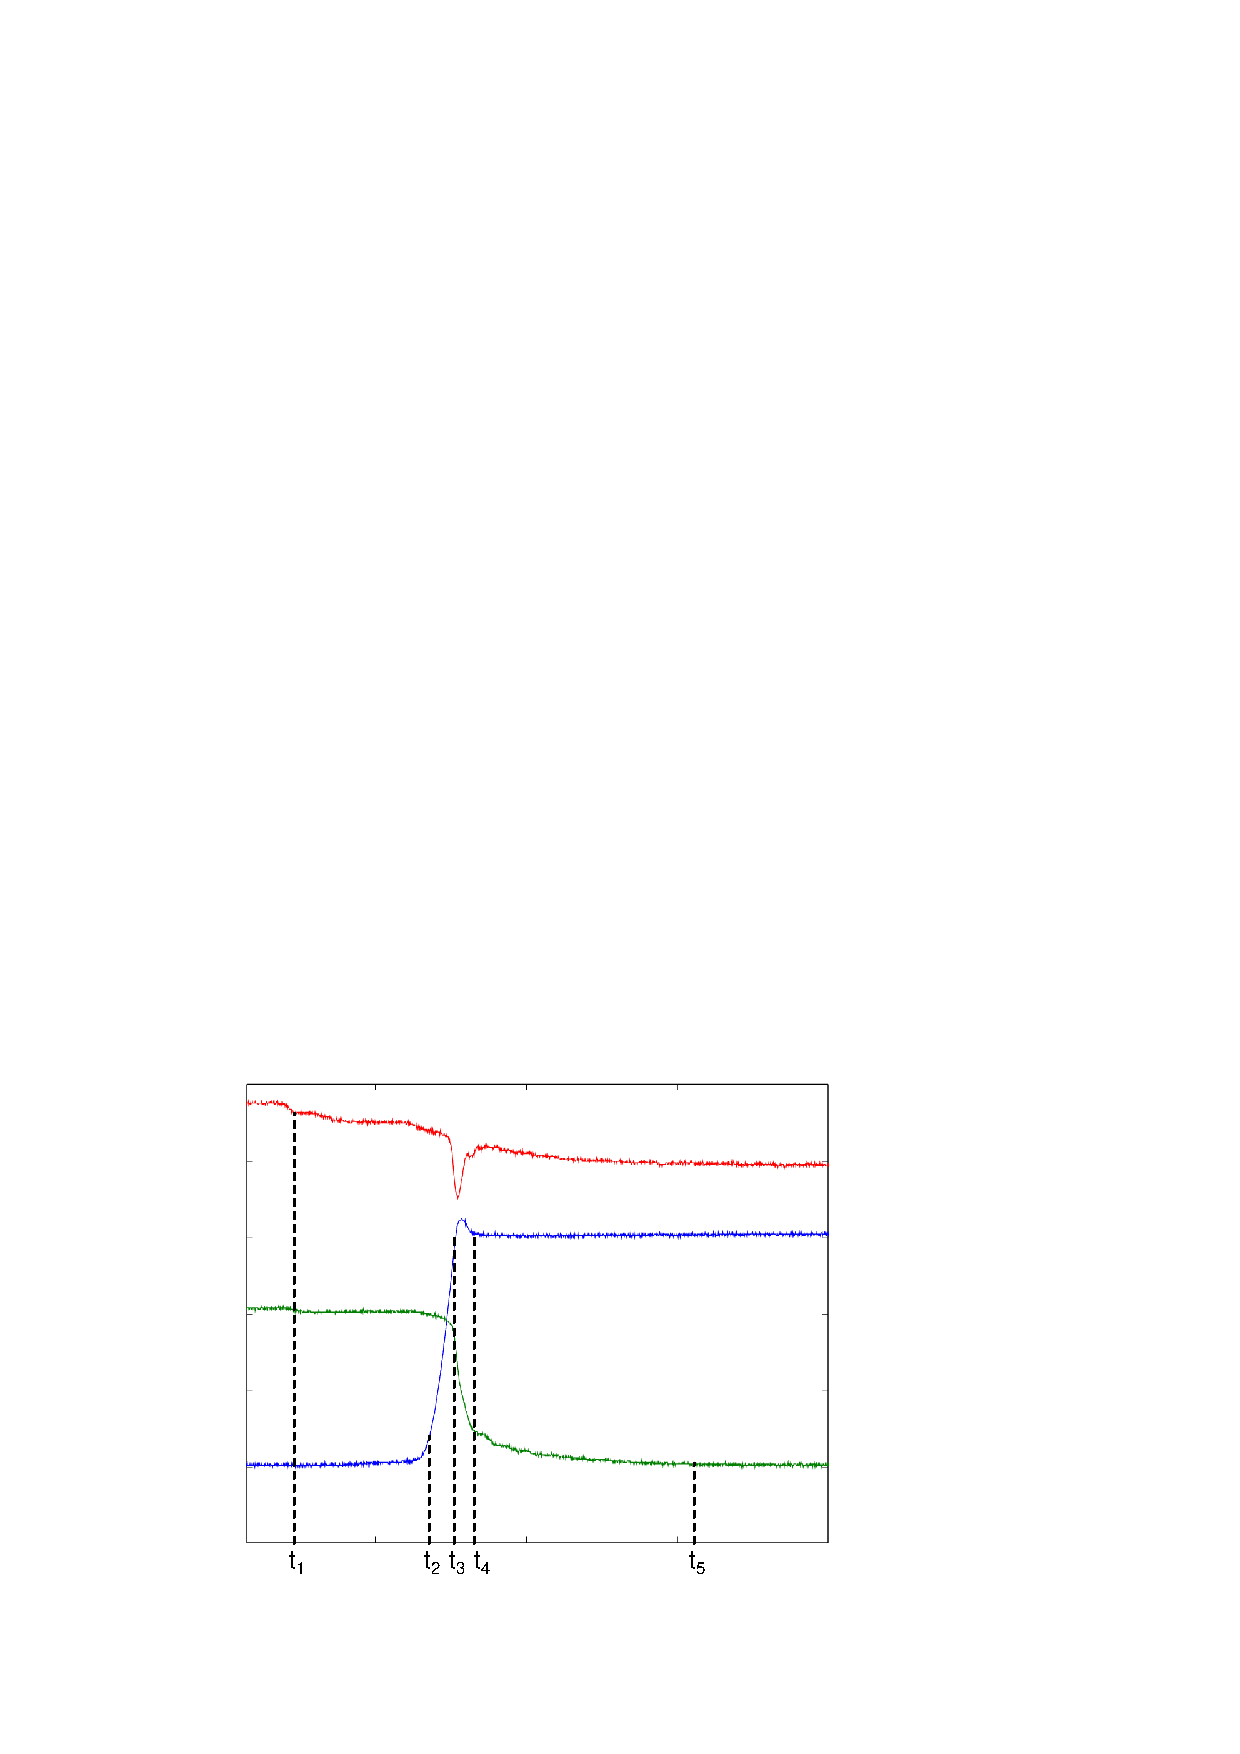
\includegraphics[width=.8\textwidth]{off.pdf}
    \caption{Definition of time intervals during turn-off action.}
    \label{fig:def_off}
\end{figure}
\begin{figure}[ht!]
    \centering
    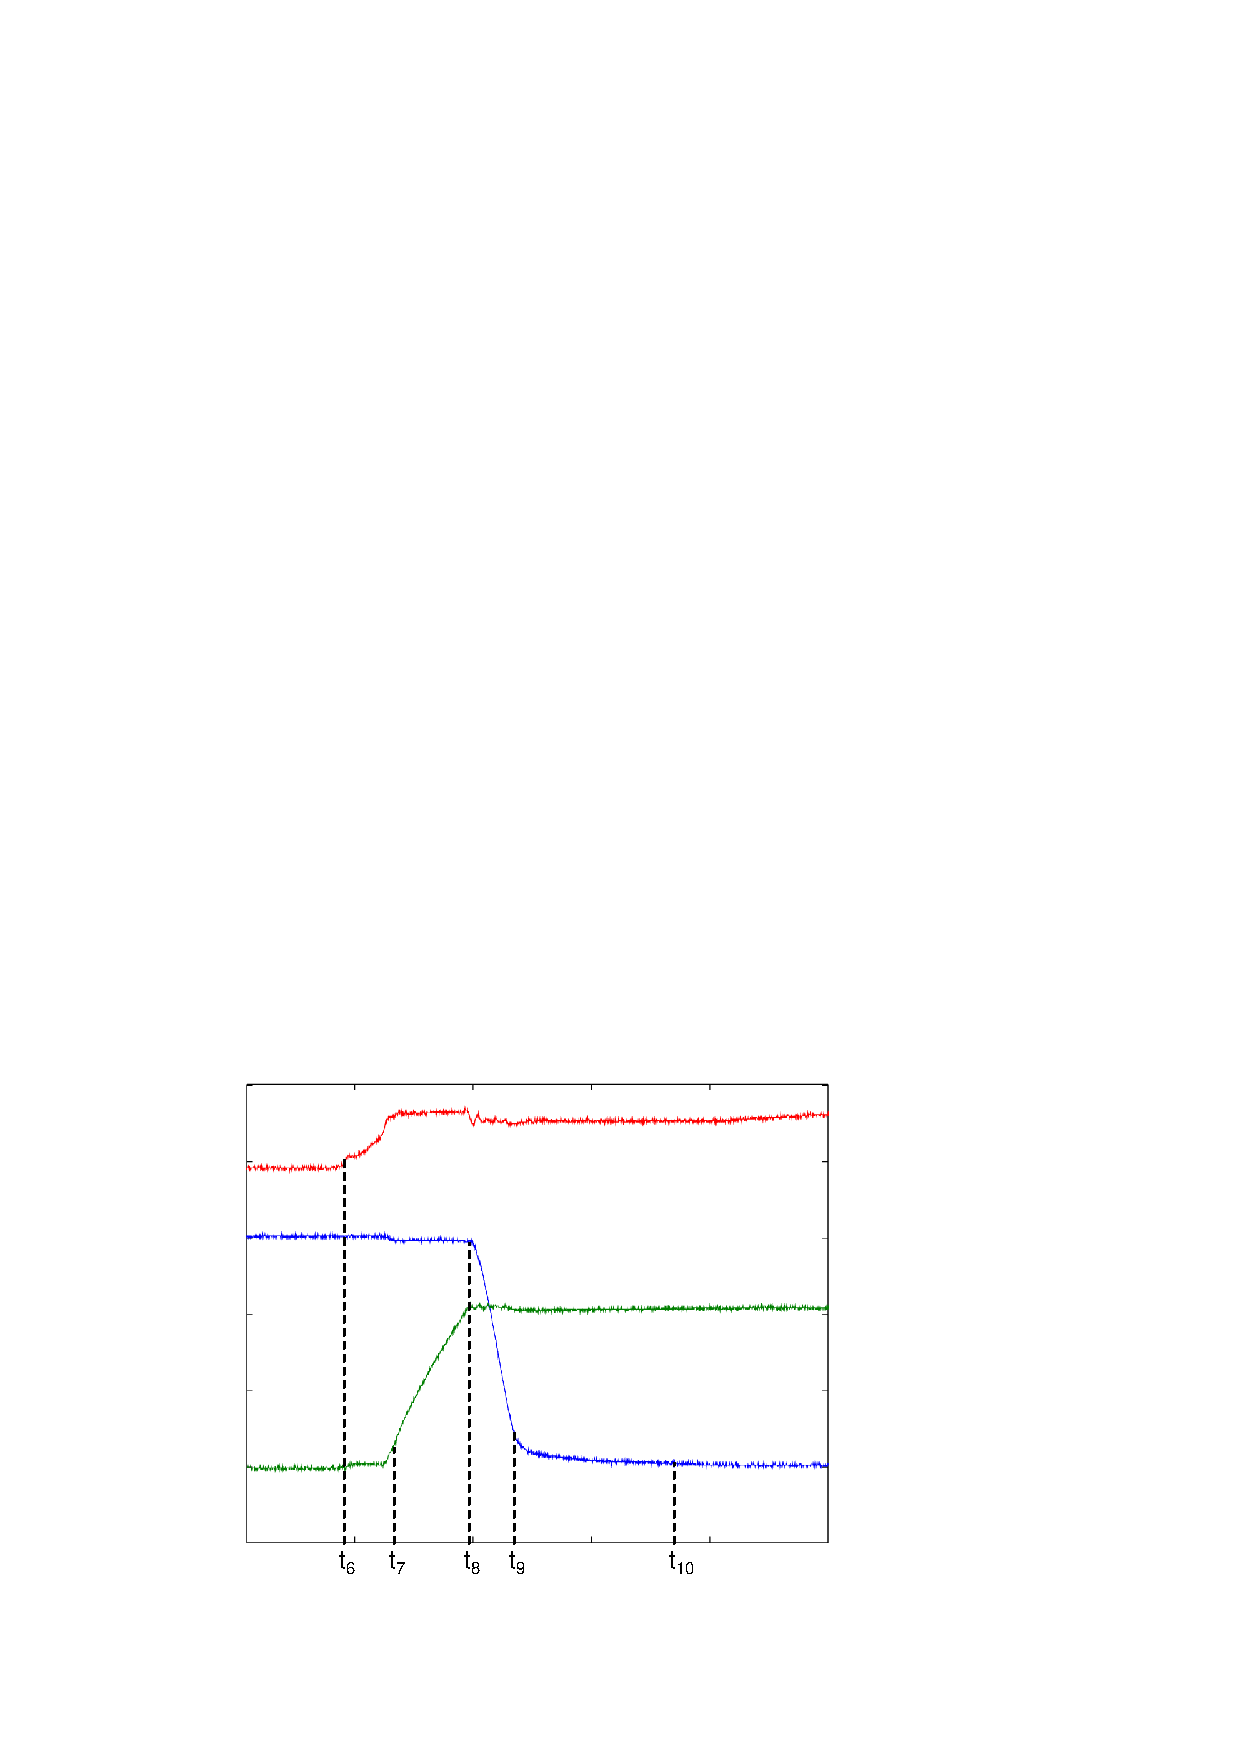
\includegraphics[width=.8\textwidth]{on.pdf}
    \caption{Definition of time intervals during turn-on action.}
    \label{fig:def_on}
\end{figure}

\myfigd{EoffmJ}{EonmJ}
\myfigd{toff}{ton}
\myfigd{didt_off_Aus}{didt_on_Aus}
\myfigd{Vpeak}{BV}

\FloatBarrier

\newpage
%\input{./kapitoly/conclusion}


\newpage
\appendix
\newpage
\part*{Appendix}
\section{Current Transformer Design Guidelines (double-pulse)}
\begin{itemize}
    \item Current transformer is unable to transfer continuous current, nor will be optimal for universal use, however the correct design yields an excellent yet inexpensive current sensor for \textit{high frequency} double-pulse test
	\newpage
    \item \textbf{Task:}
	\begin{itemize}
	    \item sum of on-times: $T_{max} = T_{on,1}+T_{on_2}$
	    \item max. current: $I_{max} = i(T_{max})$
	    \item DC-bus voltage: $V_{DC}$
	    \item ferrite core cross-sectional area: $A$
	    \item max. flux density (ferrite core): $B_{max}$
	    \item secondary turns: $N_2 = ?$
	\end{itemize}
\end{itemize}

\myfig{tr_model}{Current transformer equivalent circuit.}{tr_model}

Magnetic flux linkage:
\begin{equation}
    \Psi_2(t) = \overbrace{\Psi_0}^{=0} + \int v_2(t) \dif t
    \label{eq:Psi2}
\end{equation}

\begin{equation}
    \Psi_2 = N_2 B A
    \label{eq:Psi2=N2.B.A}
\end{equation}

\begin{equation}
    v_2(t) = \overbrace{R_2}^{R_{Cu}+R_{shunt}} \cdot i_2(t) = R_2 \cdot \frac{V_{DC}}{L_{coil}}\cdot t
    \label{eq:v2=R2.i2}
\end{equation}
$L_{coil}$ - double-pulse tester load coil.

Substituting (\ref{eq:v2=R2.i2}) into (\ref{eq:Psi2}) and combining with (\ref{eq:Psi2=N2.B.A}) yields:
\begin{equation}
    \Psi_{2,max} = \frac{R_2 V_{DC} T_{max}^2}{2 L_{coil} B_{max} N_2} = N_2 B_{max} A
    \label{eq:Psi2max}
\end{equation}

\begin{equation}
    \boxed{N_2 \geq \sqrt{\frac{V_{DC} T_{max}^2 R_2}{2 L_{coil} B_{max}A}}}
    \label{eq:N2}
\end{equation}
\textbf{note:}
\begin{itemize}
    \item $R_2 ++ \rightarrow$ limited by $B_{max}$
    \item $R_2 -- \rightarrow$ limited by shunt parasitic inductance impact
\end{itemize}

\textbf{Resulting transformation ratio:}
\begin{equation}
    v_{out} = R_{shunt} \cdot \frac{i_1}{N_2} \implies \boxed{\frac{v_{out}}{i_1}\left[ \frac{V}{A} \right] = \frac{R_{shunt}}{N_2}}
    \label{eq:tr_ratio}
\end{equation}

%\newpage
%\section{Ocvave / Matlab function library for data processing}



\section*{}

%\centering
%\vspace{60pt}
%ďzp
\end{document}
